% document style header
\documentclass[a4paper, 12pt]{config/homework}

% import default packages
\usepackage{config/defpackages}
% import custom math commands
\usepackage{config/domath}
\usepackage{pdfpages}

% end preamble
\begin{document}

% document title
\noindent
\begin{tabularx}{\textwidth}{>{\centering\arraybackslash}X>{\centering\arraybackslash}X>{\centering\arraybackslash}X}
Calvin Sprouse & PHYS489 Goal 4B & 2024 February 21\\
\midrule
\end{tabularx}

% homework problems begin
% 4B Technical writing
% Select and write a reflection on a sample of technical writing you performed for an upper division course or for some other relevant experience during your undergraduate physics program, and that you think best demonstrates the learning outcome of communicating scientific ideas effectively. Technical writing is intended to communicate primarily with those who have general expertise in the field of its topic and requires a deliberate revision, and often review, cycle. Examples of technical writing might include lab reports from upper division physics classes, grant or project proposals, technical project reports, abstracts for SOURCE or other conferences, manuscripts prepared for publication.

Attached below is my final report paper for Stellar Astrophysics. For this report we were tasked with writing a research paper on the topic we also did an oral presentation on. My topic, which aligned with my prior astronomy research, was on a particular class of star. This paper gives a general overview on what W Ursae Majoris (WUMa) stars are and their applications to astronomers. This paper synthesizes a variety of sources to give the most up to date information on WUMa stars that I could find. Of particular note were several contradictions in the literature that seemed to be based off of updated information. These contradictions came to light after I had given my oral presentation which gave rise to some reflection over how I preform my literature reviews, old sources tend to have more citations and seem more reliable but may be outdated. I noted specifically where these contradictions occur in the footnotes on the first and third page. This paper greatly enhanced my understanding of WUMa stars which would be important as I continued my research on using these variable stars to characterize the CWU 0.6m research telescope.

% include stellar report
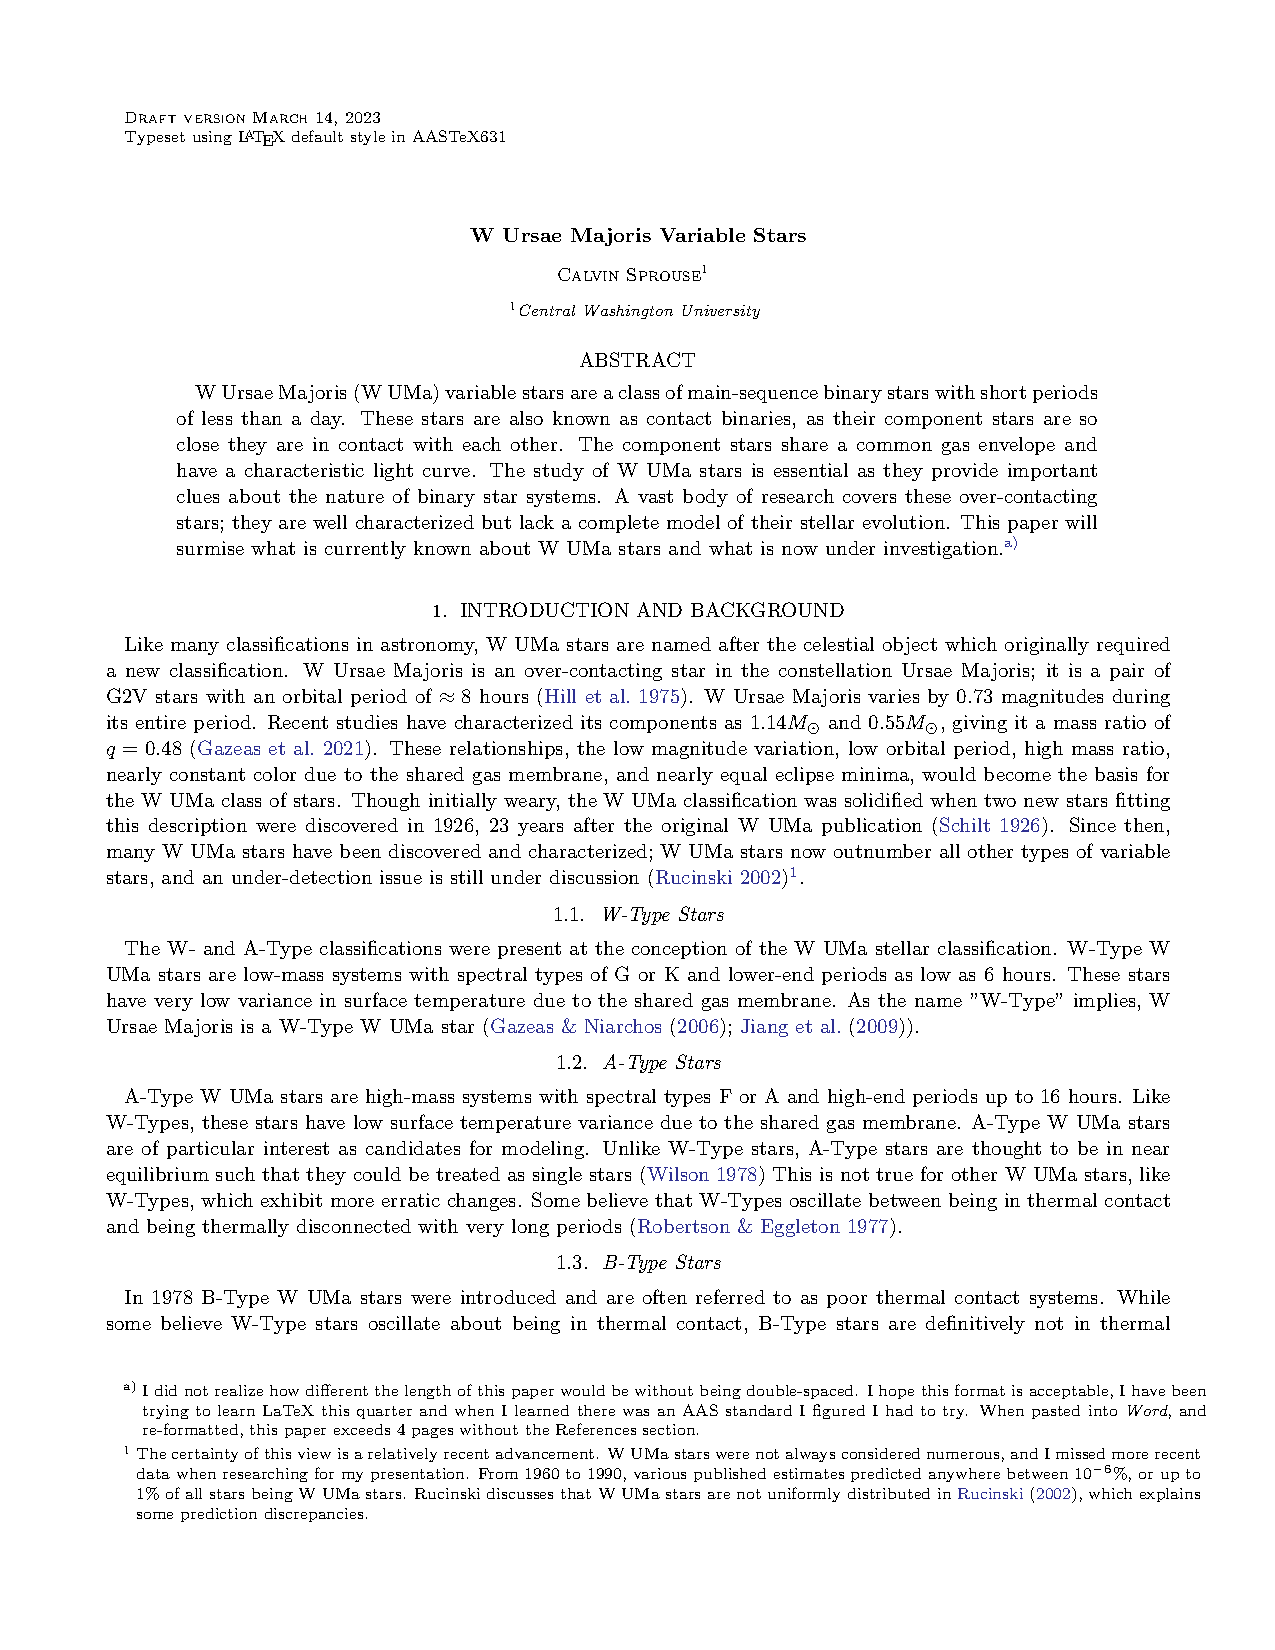
\includepdf[pages=-]{StellarAstrophysicsWUMaStars.pdf}

\end{document}
